\chapter{Intrinsic Evaluation} 
\label{ch:intrinsiceval}
\section{Introduction}
Intrinsic evaluation is to evaluate the quality of query facet generation itself. We perform intrinsic evaluation by comparing system generated query facets with ``gold standard'' query facets. Note that this evaluation can be easily extended for evaluating new models (\ie, compare the query facets generated by the new models with the existing ``gold standard'' query facets  collected before). Later, in Chapter~\ref{ch:extrinsiceval}, we will carry out an extrinsic evaluation that evaluates the quality of generated facets by their utility in assisting search.

The ``gold standard'' query facets are constructed by human annotators and used as the ground truth to be compared with facets generated by different systems. The facet annotation is usually done by first pooling facets generated by the different systems. Then annotators are asked to group or re-group terms in the pool into preferred query facets, and to give ratings for each of them regarding how useful or important the facet is.


In intrinsic evaluation, the quality of generated query facets can be measured from two aspects. (1) How well does the model generate/find correct facet terms. This can be measured by standard classification measures, such as precision and recall. (2) How well does the model groups facet terms correctly. This can be measured by standard clustering measures, such as F-measures for clustering, Purity and Normalized Mutual Information.

However, a single performance measure that combines the different aspects can be desirable in many cases. First, such a single measure provides an overall measurement for effectiveness, which is often necessary for comparing different models. Second, such a single measure can be used for tuning or training models. For example, in Chapter\todo{add ref}, we propose a method that directly using a performance measure as the training object. 

To combine the two evaluation aspects, we design a new measure called $PRF_{\alpha,\beta}$~\cite{kong2013extracting}. $PRF_{\alpha,\beta}$ combines $TP$, $TR$ and $PF$ using weighted harmonic mean, where $TP$, $TR$ and $PF$ are precision and recall for facet terms, and the F1 measure for facet term clustering. Parameters $\alpha$ and $\beta$ can be used to adjust the emphasis of the three factors for different applications.

However, $PRF_{\alpha,\beta}$ does not directly account for facet ranking performance. Dou et al.~\cite{dou2011finding} used some variations of nDCG to evaluate facet ranking. In the nDCG variation measures, system facets are mapped to truth facets, and assigned ratings according to their mapped truth facets. Then the ranked system facets are evaluated using nDCG, with the discounted gain further weighted by the precision and recall of the system facet and mapped truth facet. However, we will show that this metric can be problematic in some cases.

In the experiments of this chapter, we perform intrinsic evaluation on the different query facet extraction models described in Chapter~\ref{ch:facet}. The experimental results show that our supervised method (QF-I and QF-J) proposed in Chapter~\ref{ch:facet} significantly outperforms other unsupervised methods, suggesting that query facet extraction can be effectively learned.

In the rest of this chapter, we will first described how we collect data and perform facet annotation for intrinsic evaluation in Section~\ref{sec:ie-data}. Then, we will describe different evaluation metrics in Section~\ref{sec:ie-metrics}, including $PRF_{\alpha,\beta}$ and other existing measures. We will present our experiments for comparing different query facet extraction models in Section~\ref{sec:ie-exp}, followed by conclusions in Section~\ref{sec:ie-conclusions}. 
%The work in this chapter is completed and published~\cite{kong2013extracting}.


\section{Data} \label{sec:ie-data}
\subsection{Query}
We constructed a pool of 232 queries from different sources, including random samples from a query log, TREC 2009 Web Track queries~\footnote{http://trec.nist.gov/data/web/09/wt09.topics.queries-only}, example queries appearing in related publications~\cite{xue2011topic,wang2009mining} and queries generated by our annotators.
Annotators were asked to select queries that they are familiar with from the pool for annotating.
Overall, we collect annotations for 100 queries (see Table~\ref{tab:queries}).

\begin{table}[ht!]
\vspace{-3mm}
\centering
\caption{Query statistics}
\label{tab:queries}
\begin{tabular}{|r|r|r|} \hline
Source& \#queries& \#queries \\ 
& \ collected& \  annotated\\ \hline
query log & 100 & 30\\ 
related publications & 20 & 10\\ 
TREC 2009 Web Track & 50 & 20\\ 
annotators generated & 62 & 40\\ \hline
sum & 232 & 100\\ \hline
\end{tabular}
\end{table}	

\subsection{Search Results}
For each query, we acquire the top 100 search results from a commercial Web search engine.
A few search results were skipped due to crawl errors, or if they were not HTML Web pages.
For the 232-query set, we crawled 22,909 Web pages, used for extracting feature $listIDF$ described in Section~\ref{sec:facet-features}. For the 100 annotated queries, the average number of crawled Web pages is 98.7, the minimum is 79, both the maximum and the median are 100.

\begin{figure}[ht!]
\centering
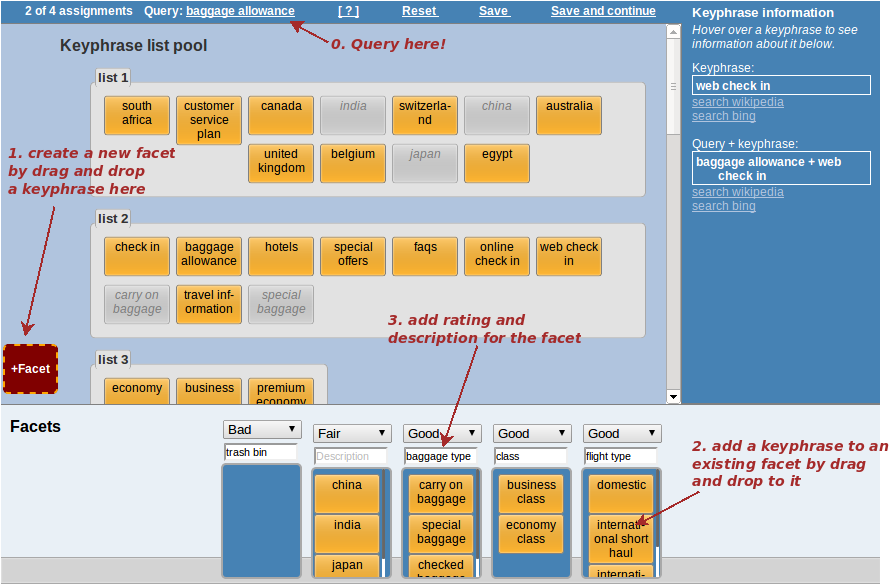
\epsfig{file=figure/facet-annotation-ui.png,scale=0.45}
%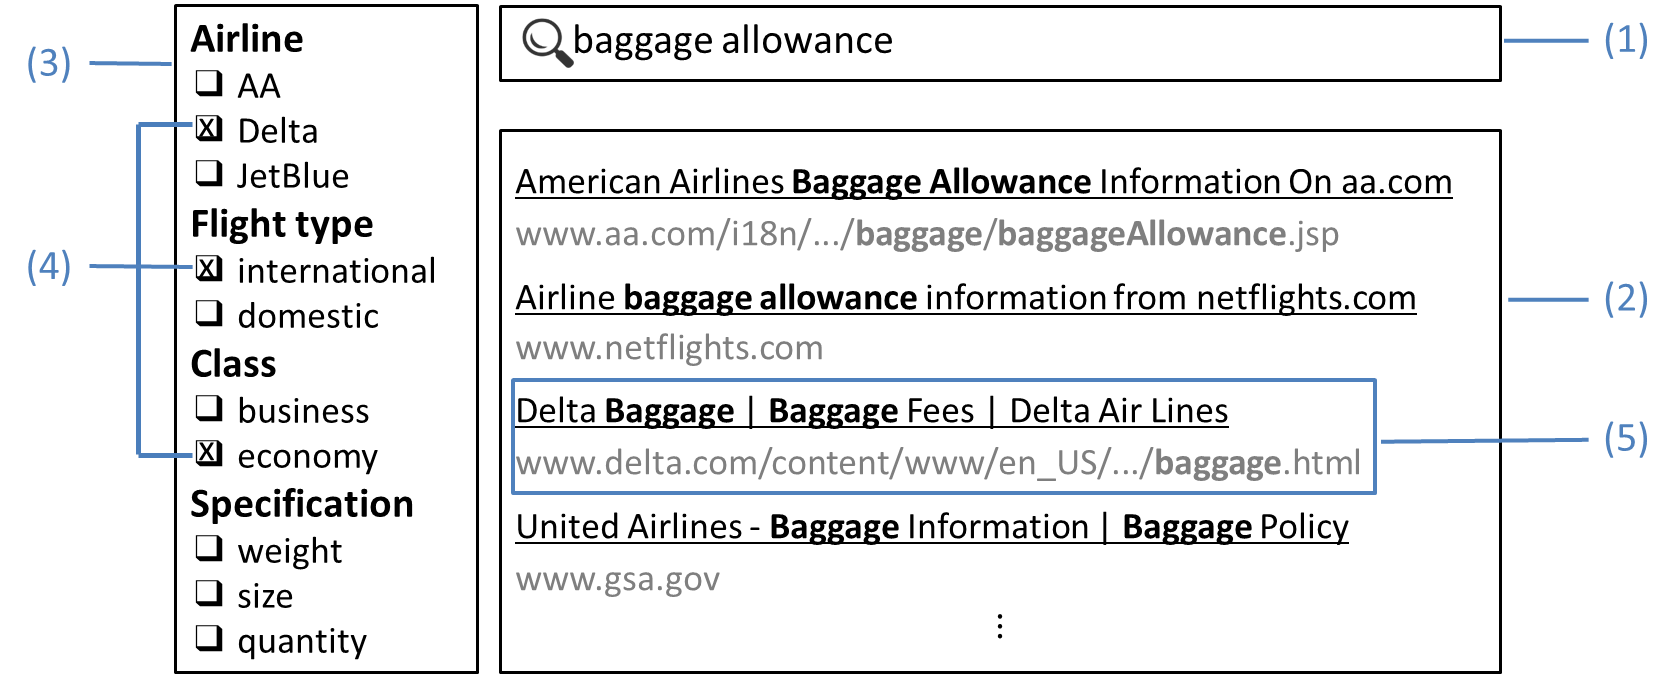
\includegraphics[scale=0.45]{figure/fws-example.png}
\caption{Annotation interface for query facet annotation.}
\label{fig:facet-annotation}
\end{figure}

\subsection{Query facet annotations}
\todo{More details about annotation description: how many annotators, etc}
We asked human annotators to construct query facets as ground truth, using the annotation interface shown in Figure~\ref{fig:facet-annotation}.
For each query, we first constructed a pool of terms by aggregating facet terms in the top 10 query facets generated by different models (corresponding to ``keyphrase list pool'' in Figure~\ref{fig:facet-annotation}), including two runs from QDM, one run from each of pLSA and LDA using top 10 list items in each query facets, and one run for our graphical model based approach. 
Then, annotators were asked to group terms in the pool into query facets for each query they selected (corresponding to step 1 and 2 in Figure~\ref{fig:facet-annotation}).
Finally, the annotator was asked to give a rating for each constructed query facet, regarding how useful and important the query facet is (corresponding to step 3 in Figure~\ref{fig:facet-annotation}). The rating scale of good=2/fair=1 is used. There are 50 query facets pooled per query, with 224.8 distinct facet terms per query. Annotation statistics for the good and fair facets, as well as the pooled facet, are given in Table~\ref{tab:annotations}. The table shows average number of facet terms per query, average number of query facets per query, and average number of facet terms per facet, for each categories (fair, good, and pooled facets).
\begin{table}[ht!]
\centering
\caption{Annotation statistics}
\label{tab:annotations}
\begin{tabular}{|l|r|r|r|} \hline
& fair & good & pooled\\ \hline
\#terms per query & 26.6 & 55.8 & 224.8\\ 
\#facets per query & 3.1 & 4.8 & 50.0 \\ 
\#terms per facet & 8.6 & 11.6 & 8.8 \\ \hline
\end{tabular}
\end{table}

\section{Metrics} 
\label{sec:ie-metrics}
Query facet extraction can be evaluated from different aspects. A good system should select ``correct'' facet terms from all the list items, therefore we use standard classification metrics, such as precision, recall and F-measures. A good system should also group those facet term correctly (i.e., in the same way as the annotators), therefore we use standard clustering metrics, such as F-measures for clustering, Purity and Normalized Mutual Information. To combine the different evaluation aspects, we design a new measure for this particular task.
\subsection{Notations} \label{sec:evalmetrics}
We continue to use notations defined in Section~\ref{sec:facet-formulation} for a query facet ($F$), a query facet set ($\mathcal{F}$) and the set of all facet terms ($T_{\mathcal{F}}$) in a query facet set. We use ``$*$'' to distinguish between system generated results and human labeled results, which we used as ground truth.
For example, $\mathcal{F}$ denotes the system generated query facet set, and $\mathcal{F}^*$ denotes the human labeled query facet set.
For convenience, we use $T$ to denote $T_{\mathcal{F}}$ in this section, omitting subscript $\mathcal{F}$.
$T^*$ denotes all the facet terms in human labeled query facet set.
We use $r_{F^*}$ to denote the rating score for a human labeled facet $F^*$.

\subsection{Effectiveness in finding facet terms}
One aspect of query facet extraction evaluation is how well a system finds facet terms. This can be evaluated using standard classification metrics as follows,
\begin{itemize}
 \item facet term precision: $T\!P=\frac{|T \cap T^*|}{|T|}$
 \item facet term recall: $T\!R=\frac{|T \cap T^*|}{|T^*|}$
 \item facet term F1: $T\!F=\frac{2|T \cap T^*|}{|T|+|T^*|}$
\end{itemize}
where the \concept{T} in measure names $T\!P$, $T\!R$, $T\!F$ stands for facet \emph{term}. It is used to distinguish the term based measures from term pair based measures as defined below. Note that these metrics do not take clustering quality into account.
%The system identified facet terms, $T$, are evaluated against human labeled ones, $T^*$, using Precision, Recall and F1.

\subsection{Clustering quality}
\label{sec:intrinsic-clustering}
To evaluate how well a system groups facet terms correctly,
similar to Dou et al.~\cite{dou2011finding}, we use several existing cluster metrics, namely, Purity, NMI/Normalized Mutual Information and pair-counting F1 measure. Here the pair-counting F1 measure treats term clustering as classification on whether each pairs of terms are in a same facet, and then combines pair precision and recall using F1 measure. We denote the pair-counting F1 measure as $P\!F$ with \concept{P} standing for term \emph{pair}.

%To avoid confusion with facet term F1, FT, we call F1 for facet term clustering \textit{facet clustering F1}, and denote it as FP (with \textit{P} standing for term \emph{pair}).

In our task, we usually have $T\neq T^*$. The facet terms in the system generated and human labeled clustering results might be different: the system might fail to include some human identified facet terms, or it might mistakenly include some ``incorrect'' facet terms. These standard clustering metrics cannot handle these cases properly. To solve this problem, we adjust $\mathcal{F}$ and $\mathcal{F}^*$ as if only facet terms in $T \cap T^{*}$ were clustered by the system, since we are only interested in how well the ``correct'' facet terms are clustered from these metrics. The adjusting is done by removing ``incorrect'' facet terms ($t \in T-T^*$) from $\mathcal{F}$, and removing missing facet terms ($t^{*}\in T^*-T$) in $\mathcal{F}^{*}$.  By this adjusting, we do not take into account the effectiveness of finding correct facet terms.

\subsection{Overall quality}
\label{sec:evalmetricsall}
To evaluate the overall quality of query facet extraction, Dou et al.~\cite{dou2011finding} proposed variations of nDCG (Normalized Discounted Cumulative Gain), namely fp-nDCG and rp-nDCG. They first map each system generated facet $F$ to a human labeled facet $F^*$ that covers the maximum number of terms in $F$. Then, they assign the rating $r_{F^*}$ to $F$, and evaluate $\mathcal{F}$ as a ranked list of query facets using nDCG.
The discounted gains are weighted by precision and/or recall of facet terms in $F$, against its mapped human labeled facet $F^*$. For fp-nDCG, only precision is used as weight, $\frac{|F^* \cap F|}{|F|}$.
For rp-nDCG, precision and recall are multiplied as weight, $\frac{|F^* \cap F|^2}{|F^*||F|}$. 

However, this these nDCG variation measures can be problematic in some cases.
When two facets $F_1$ and $F_2$ are mapped to a same human labeled facet $F^*$, only the first facet $F_1$ is credited and $F_2$ is simply ignored, even if it is more appropriate to map $F_2$ to $F^*$ (e.g., $F_2$ is exactly same as $F^*$, while $F_1$ contain only one facet term in $F^*$). Our proposed metric does not need to map facets, and thus does not have this problem.

The quality of query facet extraction is intrinsically multi-faceted. Different applications might have different emphasis in the three factors mentioned above - precision of facet terms, recall of facet terms 
and clustering quality of facet terms. We propose a metric $PRF_{\alpha,\beta}$ to combine the three factors together, using weighted harmonic mean, as follows

\begin{equation}
\label{eq:prf}
 P\!R\!F_{\alpha,\beta}(T\!P, T\!R, P\!F) = \frac{(\alpha^2 + \beta^2 + 1)}{\frac{\alpha^2}{T\!P} + \frac{\beta^2}{T\!R} + \frac{1}{P\!F}},
\end{equation}
where $\alpha,\beta \in [0,+\infty)$ are used to control the weight between the three factors in the same way as ``$\beta$'' in F-measures~\cite{van1979information}. $\alpha$ and $\beta$ can be interpreted as the importance of $T\!P$ and $T\!R$ compared to $P\!F$ respectively. More formally, we have 
\begin{equation}
\begin{split} 
 when\; \alpha &= \frac{T\!P}{P\!F} \;, \frac{\partial P\!R\!F_{\alpha,\beta}}{\partial T\!P} = \frac{\partial P\!R\!F_{\alpha,\beta}}{\partial P\!F}\\
 when\; \beta &= \frac{P\!R}{P\!F} \;, \frac{\partial P\!R\!F_{\alpha,\beta}}{\partial T\!R} = \frac{\partial P\!R\!F_{\alpha,\beta}}{\partial P\!F}.
\end{split}
\end{equation}
The intuition behind this is we want to specify the $T\!P/P\!F$ ratio at which the user is willing to trade an increment in $T\!P$ for an equal loss in $P\!F$, and similarly for $T\!R/P\!F$. For example, we can set $\alpha\!=\!2,\beta\!=\!1$ to evaluate the case where $T\!P$ is twice important than $T\!R$ and $P\!F$. When $\alpha \!=\! \beta \!=\! 1$, we omit the subscript part for simplicity, i.e. $PRF \equiv PRF_{1,1}$.

While $PRF_{\alpha,\beta}$ has the flexibility to adjust emphasis between the three factors, it does not take into account the different ratings associated with query facets. To incorporate ratings, we use a weighted version of $T\!P$, $T\!R$ and $P\!F$ in $PRF_{\alpha,\beta}$. We call the new metric $wPRF_{\alpha,\beta}$. The weighted facet term precision, recall and $T\!F$ are defined as follows.
\begin{itemize}
 \item weighted facet term precision: $wT\!P=\frac{\sum_{t \in T \cap T^*}{w(t)}}{\sum_{t \in T}{w(t)}}$
 \item weighted facet term recall: $wT\!R=\frac{\sum_{t \in T \cap T^*}{w(t)}}{\sum_{t^* \in T^*}{w(t^*)}}$ 
  \item weighted facet term F1: $wT\!F=\frac{2wP(T,T^*)wR(T,T^*)}{wP(T,T^*)+wR(T,T^*)}$ 
\end{itemize}
where $w(t)$ is the weight for facet term $t$, and assigned as follows
$$
w(t) = \left\{ \begin{array}{rl}
r_{F^*} &\mbox{ if $t \in T^*$} \\
1 &\mbox{ otherwise}
\end{array} \right.
$$
Similarly, $wP\!F$ is computed by weighting its pairwise precision and recall in the same fashion as the weighted facet term precision and recall above.
Instead of $w(t)$, we need weight for a pair of facet terms $w(t_1,t_2)$ in this calculation.
We assign weight for facet term pair $w(t_1, t_2)$ using their sum, $w(t_1) + w(t_2)$.


\section{Experiments}
\label{sec:ie-exp}
\todo{Some results need to be updated}
\todo{add more experiments testing extraction patterns, features}
\subsection{Experiment settings}
\todo{separate to multiple paragraphs}
We compare effectiveness of the five models, QDM, pLSA, LDA and QF-I, QF-J (described in Chapter~\ref{ch:facet}), on the 100-query data set.
All the models take the same candidate lists extracted/cleaned (see Section~\ref{sec:extractCandidateLists}) as input.
We perform 10-fold cross validation for training/testing and parameter tuning in all experiments and for all models (if applicable).
When training the graphical model, we standardize features by removing the mean and scaling to unit variance.
We set both of the two regularizers $\sigma$ and $\gamma$ to be 1.
%we use logistic regression implemented in scikit-learn~\cite{scikit-learn} to estimate $\mu$ and $\lambda$ in Equation~\ref{eq:lg}, and set both regularizers $\sigma$ and $\gamma$ to be 1.
There are too many negative instances ($y_i=0$, $z_{i,j}=0$) in the training data, so we stratify samples by labels with the ratio of positive:negative to be 1:3.
For QDM, we tune the two parameters used in the clustering algorithm $Dia_{max}$ (the diameter threshold for a cluster) and $W_{min}$ (the weight threshold for a valid cluster), as well as two parameters used for selecting facet terms in each facet ($S_{t|F} > \alpha |Sites(F)|$ and $S_{t|F}>\beta$).
%QDM selects facet terms as output for each query facet, when the query facets meets both of the following conditions: $S_{t|F} > \alpha |Sites(F)|$ and $S_{t|F}>1$, where $S_{t|F}$ is a score for facet term $t$, and $Sites(F)$ is the set of websites that contains any of the candidate lists in query facet $F$.
%We also tune the parameter $\alpha \in \{0, 0.02, 0.04, 0.06, 0.08, 0.1, 0.12\}$.
%Since the second condition may also prevent QDM from showing more facet term in a query facet, we also tried to exclude this condition, and tune $\alpha \in \{0, 0.005, 0.01, 0.015, 0.02\}$ in this case.
For pLSA and LDA, we tune the number of facet terms in a query facet.
% $n \in \{5, 8, 10, 11, 12, 13, 14, 15, 16, 17, 18, 19, 20\}$.
%_\{0.4, 0.5, 0.6, 0.7, 0.8\}$
For QF-I, we tune the weight threshold for facet terms, $w_{min}$, and the diameter threshold,  $d_{max}$.
%\in \{0.5, 0.6, 0.7\}
For QF-J, there are no parameter need to be tuned.
We returned top 10 query facets from all the five models in all evaluation. 
\subsection{Finding Facet terms}
\label{sec:expt}
To evaluate effectiveness in finding facet terms, we tune all the models on wTF, which combines both precision and recall, and takes into account facet term weighting.
\begin{table}[ht!]
\centering
\caption{Facet term precision, recall and F1 tuned on wTF}
\label{tab:evalclass}
\begin{tabular}{|c|c|c|c|c|c|c|} \hline
Model & TP & wTP & TR & wTR & TF & wTF\\  \hline
pLSA & 0.284 & 0.385 & 0.562 & 0.561 & 0.351 & 0.430\\
LDA & 0.292 & 0.394 & 0.595 & 0.593 & 0.364 & 0.446\\
QDM & 0.407 & 0.523 & 0.378 & 0.388 & 0.360 & 0.420\\
QF-I & 0.347 & 0.458 & \textbf{0.644} & \textbf{0.652} & 0.427 & \textbf{0.514}\\
QF-J & \textbf{0.426} & \textbf{0.534} & 0.525 & 0.526 & \textbf{0.449} & 0.511\\ \hline
\end{tabular}
\end{table}

\begin{table}[ht!]
\centering
\caption{Average number of facet terms in output per query for different models}
\label{tab:numterms}
\begin{tabular}{|c|r|} \hline
Model & \#terms/query\\  \hline
pLSA & 153.1 \\
LDA & 154.8 \\
QDM & 68.0 \\
QF-I & 153.7 \\
QF-J & 97.8\\ \hline
\end{tabular}
\end{table}

Table~\ref{tab:evalclass} shows facet term precision, recall and F1 and their weighted version described in Section~\ref{sec:evalmetrics}.
QF-I and QF-J perform relatively well for both precision and recall.
Their improvements over the other three models shown are all significant (p < 0.05, using paired t-test), except the improvements of QF-J over QDM for P and wP.
The two topic model based approaches, pLSA and LDA, have relatively high recall and low precision.
Contrarily, QDM has high precision and low recall.
This difference can be explain by Table~\ref{tab:numterms}, which gives the number of facet terms output per query from each models.
QDM only outputs 68 facet terms per query, while pLSA and LDA both output over twice that number.
One possible reason for the low precision of pLSA and LDA is that they select facet terms solely according to term probabilities in the learned topics (query facets in our case) and do not explicitly incorporate query relevance.
We find most of their facet terms are frequently-occurring list items, which are not necessary relevant to the query.
While the number of facet terms QF-I outputs is similar to pLSA and LDA, QF-I obtain much higher precision and recall, likely due to the rich set of features used.
Table~\ref{tab:fweightst} shows the five most important item features according to the absolute values of learned weights.
Not surprisingly, list TF/IDF features which are used to capture the likelihood of being a coordinate term have relatively high weights,
as well as some features that are used to capture query relevance, e.g. $TF.clueIDF$.


\begin{table}[ht!]
\centering
\caption{Top 5 item features, ranked by absolute weights}
\label{tab:fweightst}
\begin{tabular}{|l|r|} \hline
Feature & Weight \\\hline
listTF.listIDF & 2.6424 \\ 
listSF & 2.1374 \\ 
wDF & -1.0754 \\ 
TF.clueIDF & 1.0115 \\ 
SF & 0.6873 \\ \hline 
%clueIDF & -0.6705 \\ 
%DF & 0.6439 \\ 
%listTF & -0.6022 \\ 
%listDF & -0.5766 \\ 
%listIDF & -0.4896 \\ 
%snippetDF & 0.4789 \\
%length & -0.4550 \\ 
%titleDF & 0.4001 \\ 
%titleSF & -0.3961 \\ 
%snippetSF & -0.2823 \\ 
%TF & -0.2510 \\ 
%titleTF & -0.0831 \\ 
%snippetTF & -0.0136 \\ \hline
\end{tabular}
\end{table}

From Table~\ref{tab:evalclass}, we also find the the weighted metrics are usually consistent with their corresponding unweighted metric.
One exception is that QF-J performs better than QF-I in FT, but it does slightly worse than QF-J in wFT.
This is likely to be caused by the high recall for QF-I, which may include more highly rated facet terms.

\subsection{Clustering Facet terms}
Table~\ref{tab:evalcluster} shows clustering performance of the five models, which are tuned on wFP.
The improvements of QF-I and QF-J over the other three models shown are all significant (p < 0.05, using paired t-test).
pLSA and LDA do not perform well in clustering, which could be caused by data sparsity.
There are on average 5159 candidate lists per query, but only 3.9 items per list.
\begin{table}[ht!]
\centering
\caption{Facet clustering performance tuned on wPF}
\label{tab:evalcluster}
\begin{tabular}{|c|c|c|c|c|} \hline
Model &Purity & NMI & PF & wPF \\ \hline
pLSA &  0.793 & 0.524  &  0.230 & 0.229 \\
LDA  &  0.773 &  0.511 &  0.227 & 0.226 \\
QDM  & 0.871 & 0.565 &  0.367 & 0.380 \\
QF-I  &  0.843 & 0.606 &  \textbf{0.408} & \textbf{0.410} \\
QF-J  & \textbf{0.922} & \textbf{0.631} &  0.352 & 0.346 \\\hline
\end{tabular}
\end{table}

\begin{table}[ht!]
\centering
\caption{Weights learned for item pair features}
\label{tab:fweightsp}
\begin{tabular}{|l|r|} \hline
Feature & Weight \\\hline
listContextSim & 1.4944 \\
textContextSim & 0.7186 \\
listCooccur & 0.0817 \\
lengthDiff & 0.0563 \\\hline
\end{tabular}
\end{table}

The better performance in clustering for QF-I and QF-J can be explained by their incorporating factors other than list item co-occurrence information.
In Table~\ref{tab:fweightsp}, we list the weights learned for item pair features.
Besides one item co-occurrence related feature, \textit{listContextSim}, we also find that \textit{textContextSim} has a relatively high weight.
\textit{textContextSim} is used to capture the similarity of the two list items using their surrounding text, so it can help to group two facet terms together even if they might not co-occur a lot in candidate lists.
As an example, for the query \textit{baggage allowance}, we find different airlines do not co-occur a lot in candidate lists, (e.g. \textit{delta} and \textit{jetblue} only co-occur twice), but they tend to have high \textit{textContextSim} (e.g. $textContextSim(delta,jetblue)=0.81$), and are therefore grouped together by QF-I and QF-J.

\subsection{Overall Evaluation}
To compare overall effectiveness of the five models, we tune all the models on wPRF, and the results are reported in Table~\ref{tab:evalall}.
\begin{table}[ht!]
\centering
\caption{Overall performance tuned on wPRF}
\label{tab:evalall}
\begin{tabular}{|l|l|l|l|l|} \hline
Model &  wTP & wTR & wPF & wPRF \\\hline
pLSA & 0.353 & 0.630 & 0.229 & 0.309\\
LDA & 0.358 & \textbf{0.670} & 0.225 & 0.311\\
QDM & 0.523 & 0.388 & 0.253 & 0.319 \\
QF-I & 0.450 & 0.667 & \textbf{0.399} & \textbf{0.444}\\
QF-J & \textbf{0.534} & 0.526 & 0.346 & 0.417\\\hline
\end{tabular}
\end{table}

Unweighted metrics are very similar to their corresponding weighted metrics in terms of conclusions, and are omitted due to space limitation.
Results here are consistent with the results that were tuned on wFT or wFP.
pLSA and LDA have high recall, but low precision and FP.
QDM has relatively high precision, but low recall and FP. 
It has on average 68 facet terms per query as output, and fails to improve the overall effectiveness when including more facet terms in its output. 
QF-I and QF-J are among the best two models according to both PRF and wPRF.

Since wPRF does not account for facet ranking effectiveness, we also report fp-NDCG and rp-NDCG tuned on themselves in Table~\ref{tab:evalallrank}. QF-J gives the best performance for both fp-NDCG and rp-NDCG.
The improvements of QF-I and QF-J over the other three models shown in the Table~\ref{tab:evalall} and \ref{tab:evalallrank} are all significant (p < 0.05, using paired t-test), except the improvements of QF-J over QDM for wP and QF-I over QDM for fp-nDCG.
\begin{table}[ht!]
\centering
\caption{fp-nDCG and rp-nDCG tuned on themselves}
\label{tab:evalallrank}
\begin{tabular}{|l|l|l|} \hline
Model &  fp-nDCG & rp-nDCG\\\hline
pLSA & 0.250 & 0.071\\
LDA &  0.238 & 0.063 \\
QDM & 0.257 & 0.093  \\
QF-I & 0.290 & 0.157\\
QF-J & \textbf{0.336} & \textbf{0.193}\\\hline
\end{tabular}
\end{table}

\section{Conclusions} \label{sec:ie-conclusions}
In this chapter, we designed intrinsic evaluation to directly evaluate generated query facets by comparing them with human created ones. We designed an new evaluation metric that combines recall and precision of facet terms with grouping quality. Experimental results show that our supervised method (QF-I/QF-J), proposed in Chapter~\ref{ch:facet}, can take advantage of a richer set of features and outperforms other unsupervised methods.
